\begin{figure*}[!t]
  \centering
  \begin{minipage}{.5\textwidth}
  \centering
      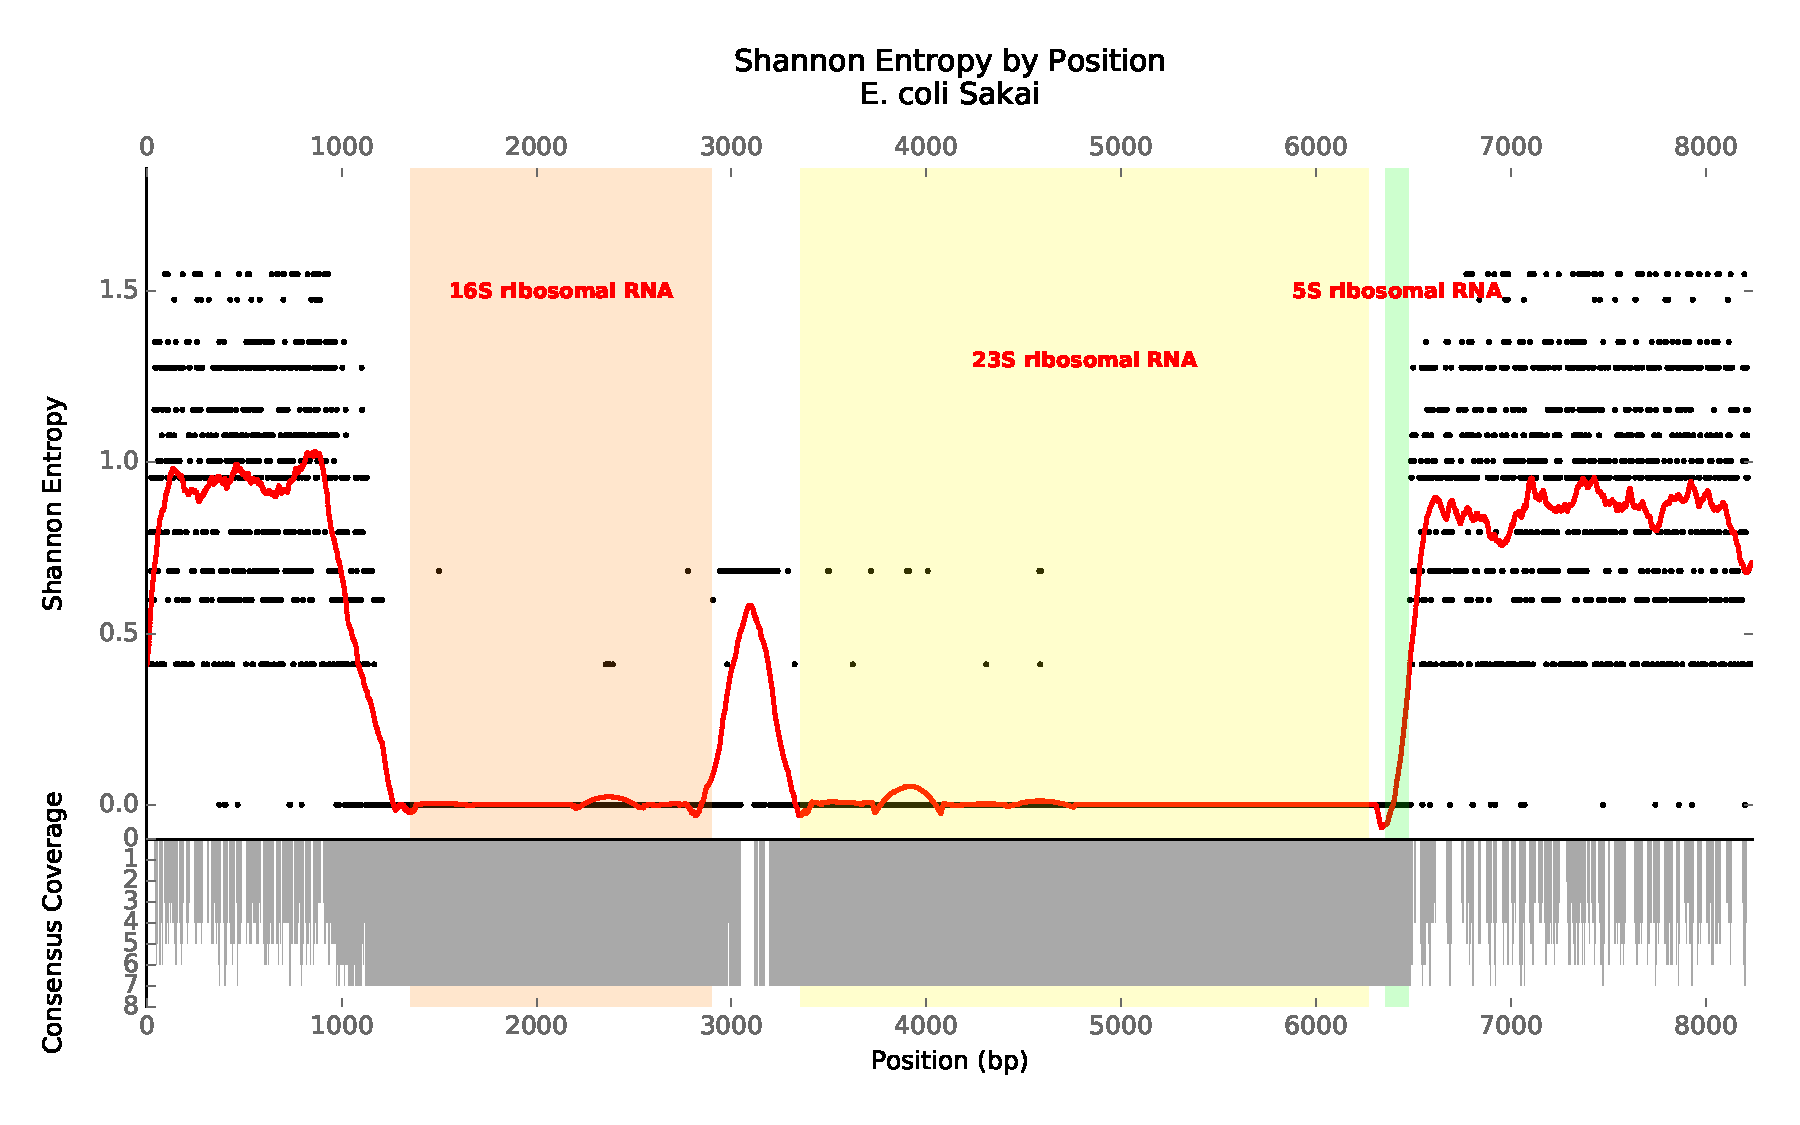
\includegraphics[width=\columnwidth]{entropy_plot}\\
      {\footnotesize \textbf{a.} All 7 rDNAs from \textit{E. coli} Sakai}
  \end{minipage}%
  \begin{minipage}{.5\textwidth}
  \centering
      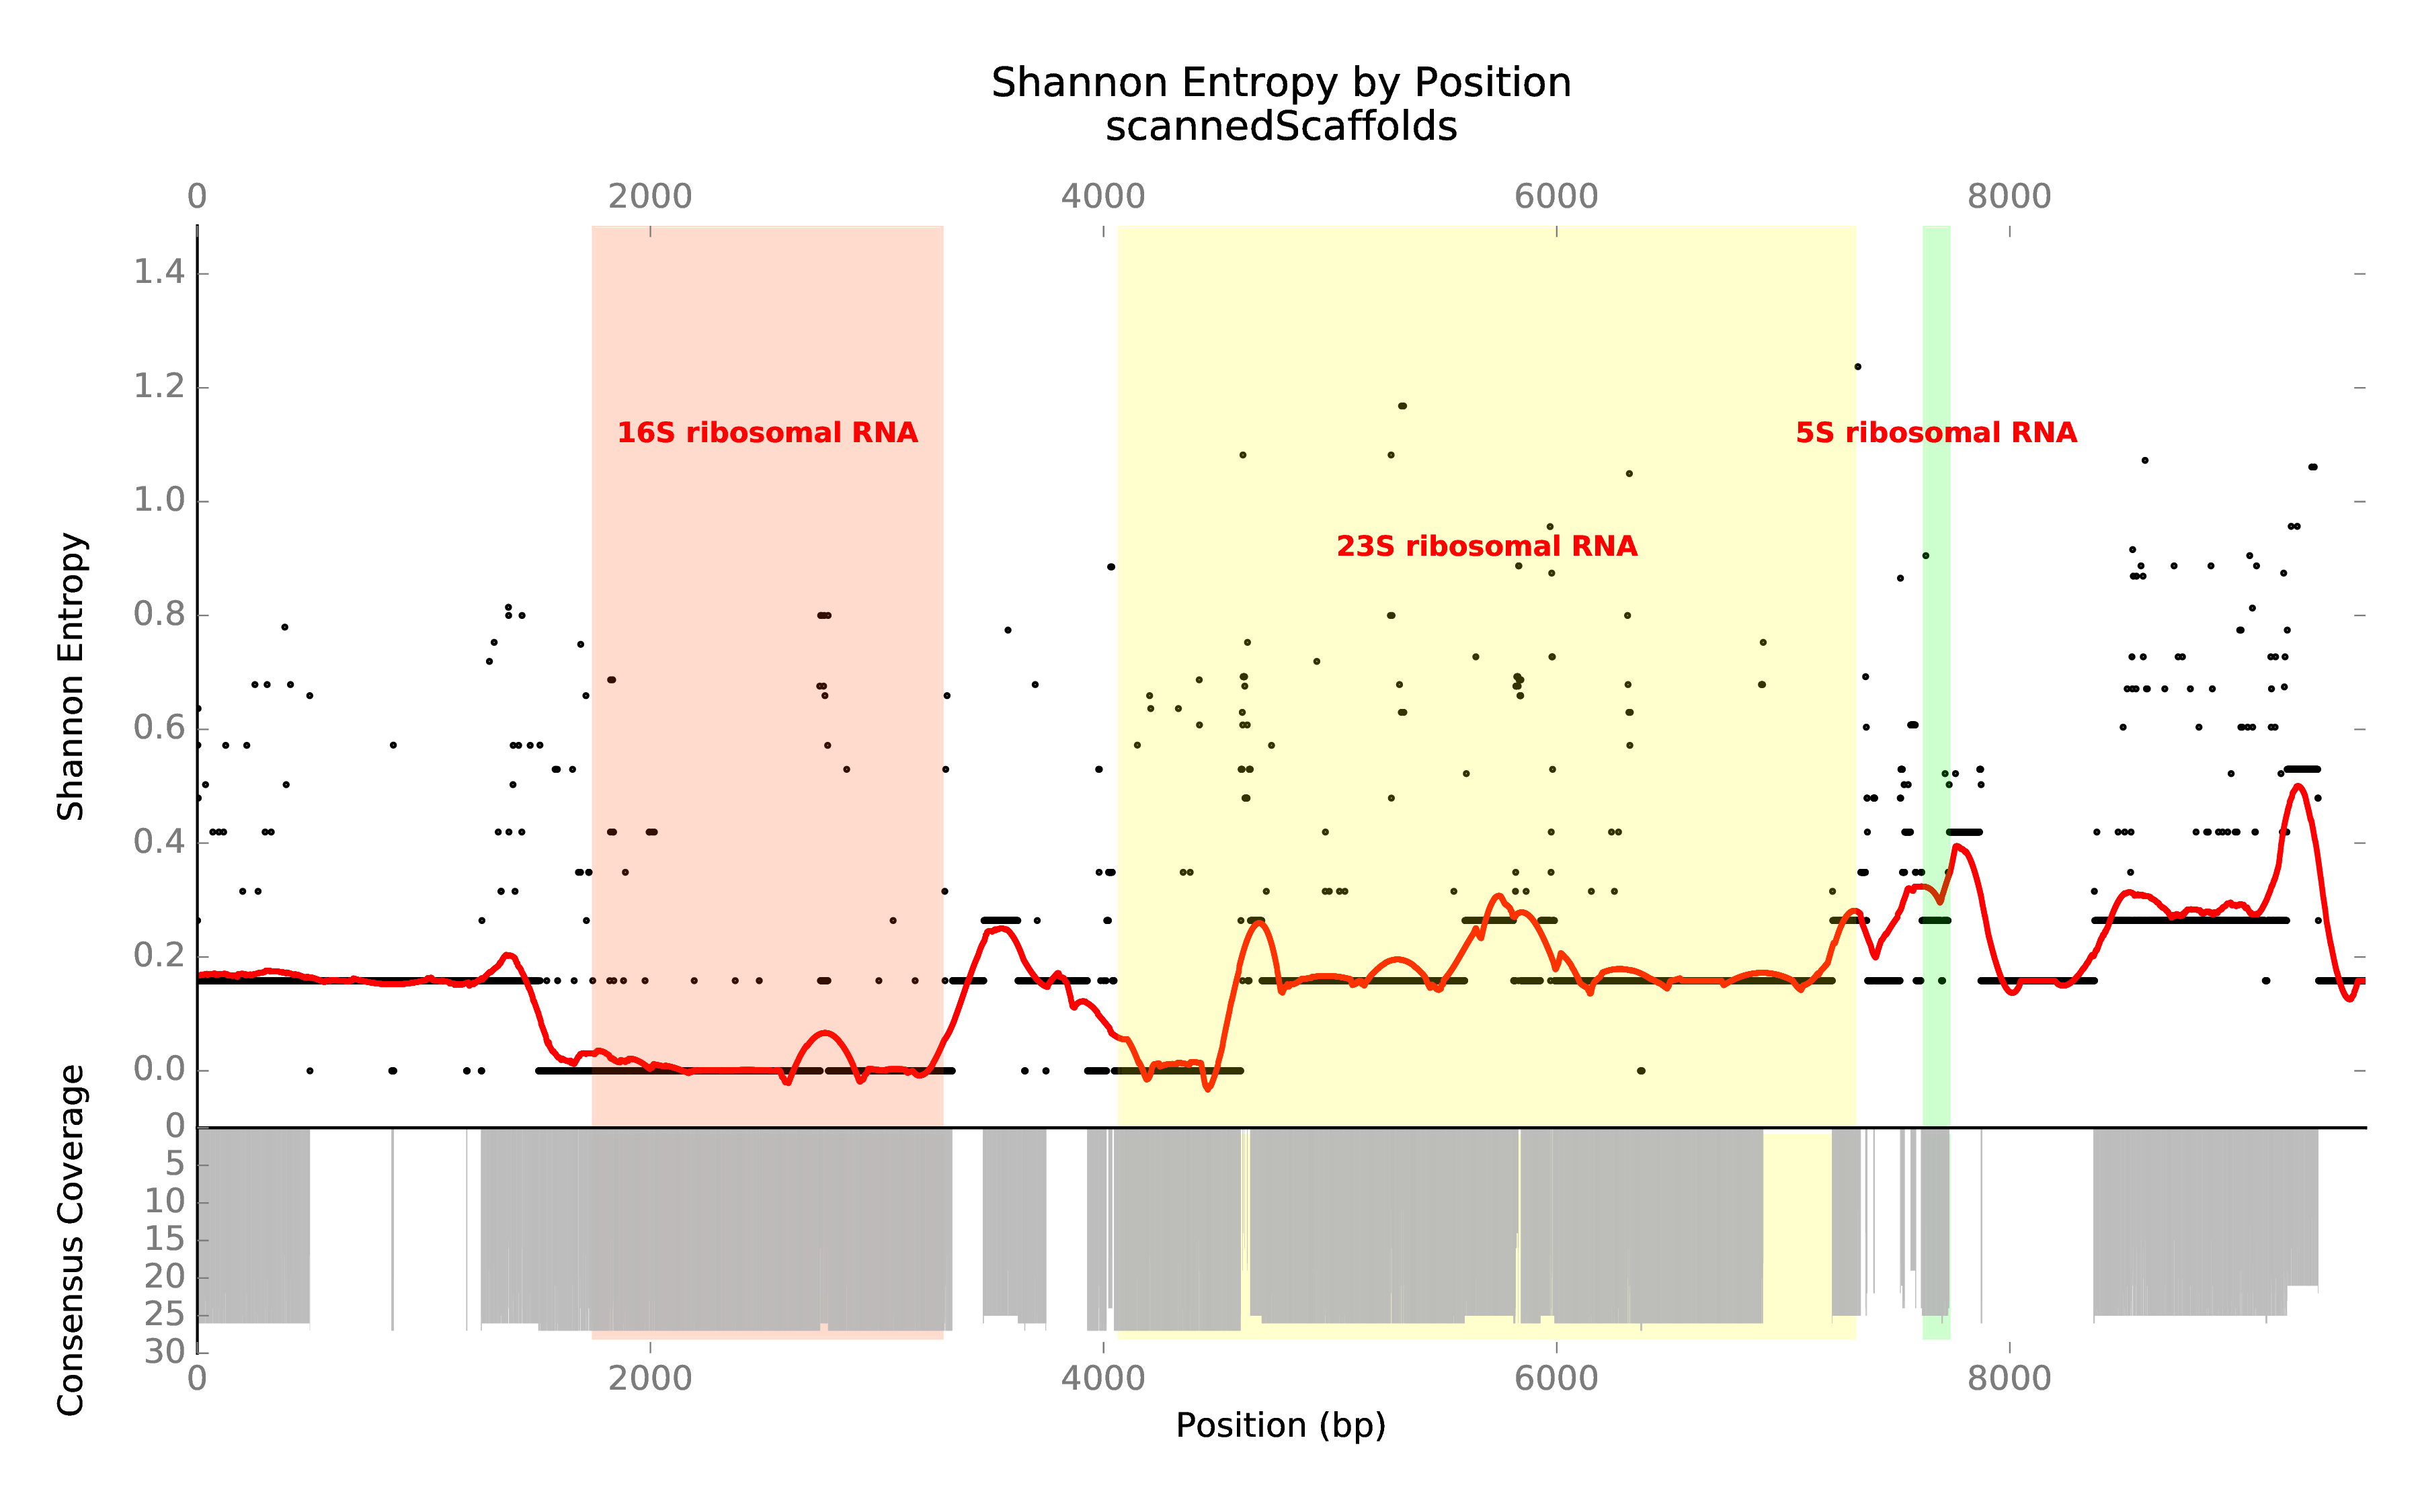
\includegraphics[width=\columnwidth]{entropy_plot_gmbH}\\
      {\footnotesize\textbf{b.} Homologues of a single rDNA locus from 25 \textit{E. coli} genomes}

  \end{minipage}%

  \caption{
    Consensus coverage depth (gray bars) and Shannon entropy (black points, smoothed with a window size of 351bp as red line) for aligned rDNA regions. For the seven \textit{E. coli} Sakai rDNA regions (a), entropy sharply increases moving away from the 16S and 5S ends of the operon. In this case flanking regions would be expected to assemble uniquely within a genome. By contrast, the rDNA regions occurring closest to homologous \textit{gmhB} genes from 25 \textit{E. coli} genomes (b) show greater conservation in their flanking regions. This indicates that flanking regions are more conserved for homologous rDNA than for paralogous rDNA operons, and implies that related genomes can be useful reference templates for assembling across these regions. Similar plots for each of the GAGE-B genomes used later for benchmarking can be found in Figure S4.
  }
  \label{fig:entropy}
\end{figure*}
